%% bare_jrnl.tex
%% V1.4b
%% 2015/08/26
%% by Michael Shell
%% see http://www.michaelshell.org/
%% for current contact information.
%%
%% This is a skeleton file demonstrating the use of IEEEtran.cls
%% (requires IEEEtran.cls version 1.8b or later) with an IEEE
%% journal paper.
%%
%% Support sites:
%% http://www.michaelshell.org/tex/ieeetran/
%% http://www.ctan.org/pkg/ieeetran
%% and
%% http://www.ieee.org/

%%*************************************************************************
%% Legal Notice:
%% This code is offered as-is without any warranty either expressed or
%% implied; without even the implied warranty of MERCHANTABILITY or
%% FITNESS FOR A PARTICULAR PURPOSE! 
%% User assumes all risk.
%% In no event shall the IEEE or any contributor to this code be liable for
%% any damages or losses, including, but not limited to, incidental,
%% consequential, or any other damages, resulting from the use or misuse
%% of any information contained here.
%%
%% All comments are the opinions of their respective authors and are not
%% necessarily endorsed by the IEEE.
%%
%% This work is distributed under the LaTeX Project Public License (LPPL)
%% ( http://www.latex-project.org/ ) version 1.3, and may be freely used,
%% distributed and modified. A copy of the LPPL, version 1.3, is included
%% in the base LaTeX documentation of all distributions of LaTeX released
%% 2003/12/01 or later.
%% Retain all contribution notices and credits.
%% ** Modified files should be clearly indicated as such, including  **
%% ** renaming them and changing author support contact information. **
%%*************************************************************************


% *** Authors should verify (and, if needed, correct) their LaTeX system  ***
% *** with the testflow diagnostic prior to trusting their LaTeX platform ***
% *** with production work. The IEEE's font choices and paper sizes can   ***
% *** trigger bugs that do not appear when using other class files.       ***                          ***
% The testflow support page is at:
% http://www.michaelshell.org/tex/testflow/



\documentclass[journal, twoside]{IEEEtran}
%
% If IEEEtran.cls has not been installed into the LaTeX system files,
% manually specify the path to it like:
% \documentclass[journal]{../sty/IEEEtran}





% Some very useful LaTeX packages include:
% (uncomment the ones you want to load)


% *** MISC UTILITY PACKAGES ***
%
%\usepackage{ifpdf}
% Heiko Oberdiek's ifpdf.sty is very useful if you need conditional
% compilation based on whether the output is pdf or dvi.
% usage:
% \ifpdf
%   % pdf code
% \else
%   % dvi code
% \fi
% The latest version of ifpdf.sty can be obtained from:
% http://www.ctan.org/pkg/ifpdf
% Also, note that IEEEtran.cls V1.7 and later provides a builtin
% \ifCLASSINFOpdf conditional that works the same way.
% When switching from latex to pdflatex and vice-versa, the compiler may
% have to be run twice to clear warning/error messages.






% *** CITATION PACKAGES ***
%
%\usepackage{cite}
% cite.sty was written by Donald Arseneau
% V1.6 and later of IEEEtran pre-defines the format of the cite.sty package
% \cite{} output to follow that of the IEEE. Loading the cite package will
% result in citation numbers being automatically sorted and properly
% "compressed/ranged". e.g., [1], [9], [2], [7], [5], [6] without using
% cite.sty will become [1], [2], [5]--[7], [9] using cite.sty. cite.sty's
% \cite will automatically add leading space, if needed. Use cite.sty's
% noadjust option (cite.sty V3.8 and later) if you want to turn this off
% such as if a citation ever needs to be enclosed in parenthesis.
% cite.sty is already installed on most LaTeX systems. Be sure and use
% version 5.0 (2009-03-20) and later if using hyperref.sty.
% The latest version can be obtained at:
% http://www.ctan.org/pkg/cite
% The documentation is contained in the cite.sty file itself.






% *** GRAPHICS RELATED PACKAGES ***
%
\ifCLASSINFOpdf
  % \usepackage[pdftex]{graphicx}
  % declare the path(s) where your graphic files are
  % \graphicspath{{../pdf/}{../jpeg/}}
  % and their extensions so you won't have to specify these with
  % every instance of \includegraphics
  % \DeclareGraphicsExtensions{.pdf,.jpeg,.png}
\else
  % or other class option (dvipsone, dvipdf, if not using dvips). graphicx
  % will default to the driver specified in the system graphics.cfg if no
  % driver is specified.
  % \usepackage[dvips]{graphicx}
  % declare the path(s) where your graphic files are
  % \graphicspath{{../eps/}}
  % and their extensions so you won't have to specify these with
  % every instance of \includegraphics
  % \DeclareGraphicsExtensions{.eps}
\fi
% graphicx was written by David Carlisle and Sebastian Rahtz. It is
% required if you want graphics, photos, etc. graphicx.sty is already
% installed on most LaTeX systems. The latest version and documentation
% can be obtained at: 
% http://www.ctan.org/pkg/graphicx
% Another good source of documentation is "Using Imported Graphics in
% LaTeX2e" by Keith Reckdahl which can be found at:
% http://www.ctan.org/pkg/epslatex
%
% latex, and pdflatex in dvi mode, support graphics in encapsulated
% postscript (.eps) format. pdflatex in pdf mode supports graphics
% in .pdf, .jpeg, .png and .mps (metapost) formats. Users should ensure
% that all non-photo figures use a vector format (.eps, .pdf, .mps) and
% not a bitmapped formats (.jpeg, .png). The IEEE frowns on bitmapped formats
% which can result in "jaggedy"/blurry rendering of lines and letters as
% well as large increases in file sizes.
%
% You can find documentation about the pdfTeX application at:
% http://www.tug.org/applications/pdftex





% *** MATH PACKAGES ***
%
%\usepackage{amsmath}
% A popular package from the American Mathematical Society that provides
% many useful and powerful commands for dealing with mathematics.
%
% Note that the amsmath package sets \interdisplaylinepenalty to 10000
% thus preventing page breaks from occurring within multiline equations. Use:
%\interdisplaylinepenalty=2500
% after loading amsmath to restore such page breaks as IEEEtran.cls normally
% does. amsmath.sty is already installed on most LaTeX systems. The latest
% version and documentation can be obtained at:
% http://www.ctan.org/pkg/amsmath





% *** SPECIALIZED LIST PACKAGES ***
%
%\usepackage{algorithmic}
% algorithmic.sty was written by Peter Williams and Rogerio Brito.
% This package provides an algorithmic environment fo describing algorithms.
% You can use the algorithmic environment in-text or within a figure
% environment to provide for a floating algorithm. Do NOT use the algorithm
% floating environment provided by algorithm.sty (by the same authors) or
% algorithm2e.sty (by Christophe Fiorio) as the IEEE does not use dedicated
% algorithm float types and packages that provide these will not provide
% correct IEEE style captions. The latest version and documentation of
% algorithmic.sty can be obtained at:
% http://www.ctan.org/pkg/algorithms
% Also of interest may be the (relatively newer and more customizable)
% algorithmicx.sty package by Szasz Janos:
% http://www.ctan.org/pkg/algorithmicx




% *** ALIGNMENT PACKAGES ***
%
%\usepackage{array}
% Frank Mittelbach's and David Carlisle's array.sty patches and improves
% the standard LaTeX2e array and tabular environments to provide better
% appearance and additional user controls. As the default LaTeX2e table
% generation code is lacking to the point of almost being broken with
% respect to the quality of the end results, all users are strongly
% advised to use an enhanced (at the very least that provided by array.sty)
% set of table tools. array.sty is already installed on most systems. The
% latest version and documentation can be obtained at:
% http://www.ctan.org/pkg/array


% IEEEtran contains the IEEEeqnarray family of commands that can be used to
% generate multiline equations as well as matrices, tables, etc., of high
% quality.




% *** SUBFIGURE PACKAGES ***
%\ifCLASSOPTIONcompsoc
%  \usepackage[caption=false,font=normalsize,labelfont=sf,textfont=sf]{subfig}
%\else
%  \usepackage[caption=false,font=footnotesize]{subfig}
%\fi
% subfig.sty, written by Steven Douglas Cochran, is the modern replacement
% for subfigure.sty, the latter of which is no longer maintained and is
% incompatible with some LaTeX packages including fixltx2e. However,
% subfig.sty requires and automatically loads Axel Sommerfeldt's caption.sty
% which will override IEEEtran.cls' handling of captions and this will result
% in non-IEEE style figure/table captions. To prevent this problem, be sure
% and invoke subfig.sty's "caption=false" package option (available since
% subfig.sty version 1.3, 2005/06/28) as this is will preserve IEEEtran.cls
% handling of captions.
% Note that the Computer Society format requires a larger sans serif font
% than the serif footnote size font used in traditional IEEE formatting
% and thus the need to invoke different subfig.sty package options depending
% on whether compsoc mode has been enabled.
%
% The latest version and documentation of subfig.sty can be obtained at:
% http://www.ctan.org/pkg/subfig




% *** FLOAT PACKAGES ***
%
%\usepackage{fixltx2e}
% fixltx2e, the successor to the earlier fix2col.sty, was written by
% Frank Mittelbach and David Carlisle. This package corrects a few problems
% in the LaTeX2e kernel, the most notable of which is that in current
% LaTeX2e releases, the ordering of single and double column floats is not
% guaranteed to be preserved. Thus, an unpatched LaTeX2e can allow a
% single column figure to be placed prior to an earlier double column
% figure.
% Be aware that LaTeX2e kernels dated 2015 and later have fixltx2e.sty's
% corrections already built into the system in which case a warning will
% be issued if an attempt is made to load fixltx2e.sty as it is no longer
% needed.
% The latest version and documentation can be found at:
% http://www.ctan.org/pkg/fixltx2e


%\usepackage{stfloats}
% stfloats.sty was written by Sigitas Tolusis. This package gives LaTeX2e
% the ability to do double column floats at the bottom of the page as well
% as the top. (e.g., "\begin{figure*}[!b]" is not normally possible in
% LaTeX2e). It also provides a command:
%\fnbelowfloat
% to enable the placement of footnotes below bottom floats (the standard
% LaTeX2e kernel puts them above bottom floats). This is an invasive package
% which rewrites many portions of the LaTeX2e float routines. It may not work
% with other packages that modify the LaTeX2e float routines. The latest
% version and documentation can be obtained at:
% http://www.ctan.org/pkg/stfloats
% Do not use the stfloats baselinefloat ability as the IEEE does not allow
% \baselineskip to stretch. Authors submitting work to the IEEE should note
% that the IEEE rarely uses double column equations and that authors should try
% to avoid such use. Do not be tempted to use the cuted.sty or midfloat.sty
% packages (also by Sigitas Tolusis) as the IEEE does not format its papers in
% such ways.
% Do not attempt to use stfloats with fixltx2e as they are incompatible.
% Instead, use Morten Hogholm'a dblfloatfix which combines the features
% of both fixltx2e and stfloats:
%
% \usepackage{dblfloatfix}
% The latest version can be found at:
% http://www.ctan.org/pkg/dblfloatfix




%\ifCLASSOPTIONcaptionsoff
%  \usepackage[nomarkers]{endfloat}
% \let\MYoriglatexcaption\caption
% \renewcommand{\caption}[2][\relax]{\MYoriglatexcaption[#2]{#2}}
%\fi
% endfloat.sty was written by James Darrell McCauley, Jeff Goldberg and 
% Axel Sommerfeldt. This package may be useful when used in conjunction with 
% IEEEtran.cls'  captionsoff option. Some IEEE journals/societies require that
% submissions have lists of figures/tables at the end of the paper and that
% figures/tables without any captions are placed on a page by themselves at
% the end of the document. If needed, the draftcls IEEEtran class option or
% \CLASSINPUTbaselinestretch interface can be used to increase the line
% spacing as well. Be sure and use the nomarkers option of endfloat to
% prevent endfloat from "marking" where the figures would have been placed
% in the text. The two hack lines of code above are a slight modification of
% that suggested by in the endfloat docs (section 8.4.1) to ensure that
% the full captions always appear in the list of figures/tables - even if
% the user used the short optional argument of \caption[]{}.
% IEEE papers do not typically make use of \caption[]'s optional argument,
% so this should not be an issue. A similar trick can be used to disable
% captions of packages such as subfig.sty that lack options to turn off
% the subcaptions:
% For subfig.sty:
% \let\MYorigsubfloat\subfloat
% \renewcommand{\subfloat}[2][\relax]{\MYorigsubfloat[]{#2}}
% However, the above trick will not work if both optional arguments of
% the \subfloat command are used. Furthermore, there needs to be a
% description of each subfigure *somewhere* and endfloat does not add
% subfigure captions to its list of figures. Thus, the best approach is to
% avoid the use of subfigure captions (many IEEE journals avoid them anyway)
% and instead reference/explain all the subfigures within the main caption.
% The latest version of endfloat.sty and its documentation can obtained at:
% http://www.ctan.org/pkg/endfloat
%
% The IEEEtran \ifCLASSOPTIONcaptionsoff conditional can also be used
% later in the document, say, to conditionally put the References on a 
% page by themselves.




% *** PDF, URL AND HYPERLINK PACKAGES ***
%
%\usepackage{url}
% url.sty was written by Donald Arseneau. It provides better support for
% handling and breaking URLs. url.sty is already installed on most LaTeX
% systems. The latest version and documentation can be obtained at:
% http://www.ctan.org/pkg/url
% Basically, \url{my_url_here}.




% *** Do not adjust lengths that control margins, column widths, etc. ***
% *** Do not use packages that alter fonts (such as pslatex).         ***
% There should be no need to do such things with IEEEtran.cls V1.6 and later.
% (Unless specifically asked to do so by the journal or conference you plan
% to submit to, of course. )


% correct bad hyphenation here
\hyphenation{op-tical net-works semi-conduc-tor}
\usepackage{amsmath}
\usepackage[pdftex]{graphicx}
\usepackage{caption}
\usepackage{textcomp}
\usepackage[labelfont=up,labelsep=newline, font=scriptsize, skip=1ex]{caption}


%Koushik's pakages%
\usepackage{amsthm}
\usepackage[bb=boondox]{mathalfa}
\usepackage[normalem]{ulem}
\useunder{\uline}{\ul}{}

%\graphicspath{ {./Figures/} }
\begin{document}
%
% paper title
% Titles are generally capitalized except for words such as a, an, and, as,
% at, but, by, for, in, nor, of, on, or, the, to and up, which are usually
% not capitalized unless they are the first or last word of the title.
% Linebreaks \\ can be used within to get better formatting as desired.
% Do not put math or special symbols in the title.
\title{The Automatic Generation of Load Test Suites and
the Assessment of the Resulting Software}
%
%
% author names and IEEE memberships
% note positions of commas and nonbreaking spaces ( ~ ) LaTeX will not break
% a structure at a ~ so this keeps an author's name from being broken across
% two lines.
% use \thanks{} to gain access to the first footnote area
% a separate \thanks must be used for each paragraph as LaTeX2e's \thanks
% was not built to handle multiple paragraphs
%

\author{Alberto Avritzer and Elaine J. Weyuker,% <-this % stops a space
\thanks{Manuscript received June 1994; revised December 1994.
A. Avritzer is with AT&T Bell Laboratories, Red Hill, NJ 07748.
E.J. Weyuker is with AT&T Bell Laboratories, Murray Hill, NJ 07974
IEEECS Log Number S95032.}% <-this % stops a space
}


% note the % following the last \IEEEmembership and also \thanks - 
% these prevent an unwanted space from occurring between the last author name
% and the end of the author line. i.e., if you had this:
% 
% \author{....lastname \thanks{...} \thanks{...} }
%                     ^------------^------------^----Do not want these spaces!
%
% a space would be appended to the last name and could cause every name on that
% line to be shifted left slightly. This is one of those "LaTeX things". For
% instance, "\textbf{A} \textbf{B}" will typeset as "A B" not "AB". To get
% "AB" then you have to do: "\textbf{A}\textbf{B}"
% \thanks is no different in this regard, so shield the last } of each \thanks
% that ends a line with a % and do not let a space in before the next \thanks.
% Spaces after \IEEEmembership other than the last one are OK (and needed) as
% you are supposed to have spaces between the names. For what it is worth,
% this is a minor point as most people would not even notice if the said evil
% space somehow managed to creep in.



% The paper headers
\markboth{IEEE TRANSACTIONS ON AUDIO,~SPEECH,~AND~LANGUAGE~PROCESSING,~VOL.~16, NO.~9,~SEPTEMBER~1995}
{IEEE TRANSACTIONS ON AUDIO,~SPEECH,~AND~LANGUAGE~PROCESSING,~VOL.~16, NO.~2,~FEBRUARY~2008}
\markright{YANG \MakeLowercase{\textit{et al.}}: REGRESSION APPROACH TO MUSIC EMOTION RECOGNITION}
% The only time the second header will appear is for the odd numbered pages
% after the title page when using the twoside option.
% 
% *** Note that you probably will NOT want to include the author's ***
% *** name in the headers of peer review papers.                   ***
% You can use \ifCLASSOPTIONpeerreview for conditional compilation here if
% you desire.




% If you want to put a publisher's ID mark on the page you can do it like
% this:
\IEEEpubid{0098-5589/95\$04.00 \textcopyright\ 1995 IEEE}
% Remember, if you use this you must call \IEEEpubidadjcol in the second
% column for its text to clear the IEEEpubid mark.



% use for special paper notices
%\IEEEspecialpapernotice{(Invited Paper)}


\IEEEaftertitletext{\vspace{-2\baselineskip}}

% make the title area
\maketitle

% As a general rule, do not put math, special symbols or citations
% in the abstract or keywords.
\begin{abstract}
Three automatic test case generation algorithms intended to test the resource allocation mechanisms of telecommunications software systems are introduced. Although these techniques were specifically designed for testing telecommunications
software, they can be used to generate test cases for any software
system that is modelable by a Markov chain provided operational
profile data can either be collected or estimated. These algorithms
have been used successfully to perform load testing for several
real industrial software systems. Experience generating test suites
for five such systems is presented. Early experience with the algorithms indicate that they are highly effective at detecting subtle
faults that would have been likely to be missed if load testing had
been done in the more traditional way, using hand-crafted test
cases. A domain-based reliability measure is applied to systems
after the load testing algorithms have been used to generate test
data. Data are presented for the same five industrial telecommunications systems in order to track the reliability as a function of
the degree of system degradation experienced. \\

\IEEEKey
\textit{Index Terms\(-\)}Automatic test case generation, software testing,
reliability assessment, Markov chains.
\end{abstract}

\section{Introduction}
\IEEEPARstart{A}{MAJOR} challenge for organizations that develop software for industrial purposes is to determine ways to comprehensively test the resource allocation mechanisms associated
with the software in a cost effective manner. Although there is
a great deal of literature describing testing strategies that address the functionality of the software under test, there is very
little literature describing approaches to this related, but distinct, problem.

In this paper, we therefore address several issues related to
the testing of resource allocation in systems \textit{after} the system
functionality has been thoroughly tested. The algorithms we
propose are \textit{black-box} testing techniques since they do not rely
at all on details of the implementation. They are examples of
what are typically called \textit{load testing} strategies, since they
assess how the system performs under a, given ‘‘load.’’ The
strategies we introduce are based on an \textit{operational profile}
which describes the expected workload of the system once it is
operational in the field \cite{b7}. The operational profile for a telecommunications system typically includes the following types
of information: the number of different types of calls, the average service demands and probability distribution for each type
of call, and the average external arrival rate and probability
distribution for each call type. If the same types of calls can be routed through different locations (so-called \textit{service centers}),
then the routing probabilities between service centers for each
call type would also typically be included. We have generally
found the needed operational profile information to be readily
available for the projects with which we have worked.

In the research literature for local area networks (LANs), a
distinction is frequently made between \textit{hard failures} and soft
failures. A hard failure is said to occur when there is a problem that leads to no traffic through the network. This might be
due to such events as the severance of a network cable leading
to a physical discontinuity in the network, a power failure, or a
failure of one or more major network components such as a
router. The analogue of a hard failure for a software system is
a system crash. In such a c?se, the system is totally unavailable
until some intervention has been taken.

\textit{A soft failure}, in contrast, is said to occur in a network when
the network’s performance has degraded. These performance
degradations might be either transient or permanent. For example, intermittent electrical problems might lead to transient
failures which disappear dnce the cause of the problem has
been removed. For a software system, this type of intermittent
soft failure might happen when a burst of activity occurs, requiring more resources than the system has available. In the
case of telecommunications systems, if the total number of
active calls plus the number of incoming calls exceeds the
system’s capacity, some calls will be lost. Once the load decreases, the system resumes normal operation. In a typical
telecommunications system, it is extremely important that this
type of failure does not occur. For this reason, telecommunications systems are typically designed with a very substantial
amount of excess capacity so that the probability of call loss or
blockage in a properly functioning system is very low. This
means that this type of intermittent soft failure is very unusual
in the systems we will be considering because the systems
have been designed explicitly to prevent this type of failure.
 
 If a soft failure is permanent, then once the degradation has
begun, the network remains in a degraded state until appropriate intervention has been taken to restore acceptable performance. The analogue of a permanent soft failure for software is
a problem that leads to a degradation of the software that does
not abate when the load decreases.

\IEEEpubidadjcol
When doing load testing of telecommunications systems, it
is extremely unusual to see a hard failure, and as mentioned
above, systems are typically designed to prevent soft transient
failures. In fact, at this stage it is unusual to see \textit{any} type of
failure, but among the few failures that we see, the typical failure is a permanent soft failure. That is, a failure typically consists of a situation in which the service provided to some users
is not entirely acceptable because the system has degraded so
that full capacity is not available. In this case, calls (or users)
are lost to the system, even though there are ample resources
available. In such a situation, once the system enters this type
of faulty state, the system typically continues to degrade, losing more and more users, or in our environment, preventing
the completion of increasing numbers of calls. We refer to this
situation as a \textit{smoothly degrading} system. It is this type of
system and failure that we consider in this paper, and the primary goal of the testing approach that we present here is to
identify and fix these types of faults, thereby preventing the
associated soft failures.
\IEEEpubidadjcol

In \cite{b1}, a new automatic test case generation strategy for performing load testing for systems that can be modeled by
Markov chains was proposed. In the current paper, we introduce two additional variants of these algorithms. These new
strategies increase the class of detectable faults by examining
not only the amount of resources allocated, but also the order
of that allocation. For each of the three algorithms, a domain based reliability measure is defined.

The algorithms were used to generate test suites for five industrial telecommunications projects, and our experience is
reported. Preliminary results are extremely encouraging, and
are described in Sections 1II.B and 1V.B. In Section V we also
consider interesting uses of the reliability computation. 
\section{The Model}
In this section we include a very brief introduction to
Markov processes as necessary to understand our test case
generation approach. A much more thorough description of
this background material is available in \cite{b5}. We also provide a
brief introduction to the terminology needed to understand the
application domain in which we have applied our algorithms:
telecommunications systems.

Let \(X\) be a set of random variables.\(X\) = \{\(x_i\)\}  is said to form a \textit{Markov chain}  provided that the probability that the next state
is \(x_{m+1}\) is independent of everything other than the current
state, \(x_m\). Thus, the only way that the past history of the process
can affect the future is through the current state. This is sometimes known as the \textit{memory less property}.

In the telecommunications application domain, a typical
state might represent an n-tuple of call types, with the \textit{i}th element of the n-tuple, \(m_i\),  representing the numbers of active
calls of type \(i\). If the system is in state (\(m_l, m_2, ..., m_i, ..., m_n,\)),and a new call of type \(i\), is placed, the system enters state (\(m_1, m_2, ...,m_i+1, ..., m_n\)). There are typically two types of transitions in these systems: call arrivals and call completions. Associated with each transition is a value representing the call
arrival or completion rate.

The \textit{holding time} e for a call includes all the time during
which the call is active, including all the time that the caller is
using the system. The \textit{call arrival rate }is simply the average rate at which calls of a given type enter the system. Similarly,the call \textit{completion or departure rate} is the rate at which calls leave the system. This is equal to the inverse of the average
call holding time for that call type, times the number of calls of the given type in the state. Thus, if the average call holding time is two minutes for a call of a given type, then the departure rate for that call type from a state containing \(N_i\) calls of
that type is \(\frac{N_i}{2}\). \textit{Call blocking} is said to occur if a call cannot be completed because all circuits are already allocated to other calls.

The only continuous-time distribution that exhibits the
memoryless property is the exponential distribution \cite{b5}. We
therefore require that the average time for a transition out of a state be exponentially distributed: We assume that each call type forms an independent Poisson process with a specified arrival rate, and that call holding times are exponentially distributed. It is generally agreed that most telecommunications systems can be accurately modeled in this way.

One special case of a Markov chain is known as a \textit{birth-death process}, which requires that the only state transitions
that can occur are between so-called \textit{neighboring states}. That
is, the states can be numbered in such a way that if \(x_n = i\), then \(x_{n+l}\) must be \(i, i - 1,\) or \(i + 1.\) Viewed from the perspective of a single call type, the systems we consider can be modeled in this way, and we approximate the behavior of actual states of our system which represent vectors of call types by considering the product of these factor solutions.

The general steady-state solution for birth-death queuing
systems is derived in \cite{b5}. 

The solution for this type of system for a single call type is given by: 
\begin{equation}
    p_k = \frac{\lambda_0\lambda_1...\lambda_{k-1}}{\mu_1\mu_2...\mu_k}
\end{equation}
where \(p_i\) denotes the probability that there are \(i\) calls of the specified type, \(\lambda_i\) denotes the call arrival rate when there are \(i\) active calls of the specified type, and \(\mu_i\) denotes the call
completion rate when there are \(i\) active calls of the specified type.

Equation (1) can be rewritten as: 
\begin{equation}
    p_k=\frac{\lambda_{k-1} }{\mu_k} p_{k-1}
\end{equation}
that is, the probability of having \(k\)  calls of a given type at a given time is equal to the probability of having \(k - 1\) calls of that type, times the ratio of the call arrival rate when there are \(k - 1\) calls in the system and the call departure rate when there are \(k\) active calls of the given type.This ratio represents the
expected number of active calls of the given type. It follows
immediately from (2) that if  $ \frac{\lambda_{i-1}}{\mu_i}<1 $   , $  p_i < p_{i-1} $ . The condition for the existence of equilibrium probabilities is that
there exists a $k$ , such that for all   $ i \geq k $ , $ \frac{\lambda_{i-1}}{\mu_i}<1 $ . This observation is important as it will frequently allow us to truncate the
number of states considered by the algorithms presented in the next section.

In Section 111 we describe a family of three test generation
algorithms. In the first algorithm, all faults under consideration
are entirely associated with a state. The second algorithm also
considers faults which might be associated with individual
transitions between states, while the third algorithm considers
subpaths of varying lengths from a given state, back to itself.
Note that when we assume that the system is being modeled by
a Markov chain, we do so \textit{only} to derive the steady-state probability distribution for the states, and not for the determination
of potential faults. Of course, it may be the case that faults
occur that are dependent on the explicit path exercised, rather
than being entirely state dependent, and it is for that reason
that the second and third algorithms are introduced.

The proposed approach is to generate only those software
states, and hence associated test cases, that have probabilities
greater than a heuristically computed $\varepsilon$ , and thus represent
software states that are the most likely to be reached in the
field. Letting $K$ denote the number of states with probability
greater than $\varepsilon$ , it follows that $\varepsilon$  and $K$ are related by the           
steady-state probability distribution, and by the total number of
calls, $M$, generated by the $K$ test cases. We typically start with
a small value for $\varepsilon$  and tune it until the number of test cases is
approximately equal to a number indicated by the testers as
feasible to perform. This tuning of  $\varepsilon$  is done using a binary search.

The structure of the problem leads to the following recursion: generate the current state and all states derived from it by
adding one more outstanding call of type $x$, until the test case
probability is less than $ \varepsilon $.On return, increment to the next type
of call, and recursively repeat the procedure.
To simplify the description of the algorithms, we assume
that call types are sorted by $\frac{\lambda_i}{\mu_i}$. That is, the call type with the
greatest expected number of active calls will be call type 1, the
second highest will be type 2, and so on. 

\section{THE MARKOV STATE TESTING APPROACH}
Deterministic Markov state testing is a test case generation
and execution approach designed for performing load testing
for telecommunications software according to an operational
profile. Note that although we generally speak of applying our
test case generation algorithms to test the software of telecommunications systems, our procedure is suitable for any
software systems that meet the above-outlined assumptions,
with the state appropriately defined. In Section III.B, we will
present our experience applying these algorithms to perform
load testing for five industrial software telecommunications
systems. Of these five projects, only Project 1 has call types as
the primary operations. This should give the reader a feel for
the range of applications for which our algorithms can and
have been used. Throughout the paper, however, we will continue to speak about telephone calls as the primary operations,
since this is a concrete application that is easy for most readers
to conceptualize.

A central problem associated with the type of software we
consider here is that even for systems with a relatively small number of call types, and modest upper bound on the number
of calls that the system can handle, there will typically be a
huge number of distinct states. Since each state of the Markov
chain corresponds to one or more test cases for load testing,
this translates to a vast amount of required testing if total coverage of the state space is required. For a system that can handle k distinct types of calls, and a maximum of n calls, the
system would contain   
$\begin{pmatrix}
n+k \\
n
\end{pmatrix}$  states. Thus, a system that can
handle a maximum of 24 calls of five distinct types would
have a total of 1 18,755 Markov states. To test every state once
would require a total of 5,938 hours of testing, assuming three
minutes holding time for each call. If the maximum number of
calls were increased to 500, there would be a total of
268,3 18,178,226 Markov states requiring over 13,000,000,000
hours of testing assuming three minutes holding time. Since
this clearly requires a prohibitive amount of resources, some
way of intelligently selecting a relatively small subset of these
potential test cases must be developed. 

Our algorithms therefore involve a recognition that faults
associated with those states that correspond to the most likely
states to be executed, translate into failures that are most likely
to be encountered in the field, and hence situations that are
most likely to be problematic. Thus, in order to minimize observed field failures, our first test case generation approach
stresses the testing of those states of the Markov chain that
have the greatest likelihood of being encountered. Note that a
Markov chain can be represented by a graph, and hence when
we speak of edges, paths, or cycles, we are really referring to
the state transitions and sequences of transitions.

By limiting our first test case generation algorithm to the
selection of at most one test case per state, there is a tacit assumption being made that the only faults of interest are those
that are directly associated with a particular state, and not the
edge or path traversed to arrive at the state. Looking at this
from a different perspective, this can be viewed as an assumption that all paths to a state are equally likely to be faulty. Although we would certainly not argue that this is a reasonable
assumption for earlier stages of (functionality) testing, experience has shown that this is frequently reasonable for performing load testing. Typical faults that we expect to be detected by
this approach involve improper allocation of resources such as
buffers, demons, or memory, leading to a loss of calls, or a
store and forward deadlock in a client/server environment.

If in addition to testing state definitions, it is determined
that the edge taken to the state should also be tested at this
stage, we provide a second algorithm that generates in order,
all state transitions such that the product of the state probability and the call arrival rate is greater than $\varepsilon$. . A typical type of
fault that might be detected by this algorithm is a degradation
of the number of calls that can be accepted by the system. This
is a common type of problem for telecommunications systems.
For example, data from eleven test sessions for an actual industrial project are shown in Table I. The total number of client and subscriber calls made during the run, and the call
completion rate achieved are shown. These call completion
rates clearly identify a major degradation in the system avail- \vspace{5cm} 

ability, which is visible to the user as calls unable to complete.
For this project, originally described in [l], the system was
rebooted after test sessions three and nine in order to restore
the system to full capacity as a temporary fix. Once the problem was identified using our approach to the generation of
load test suites, however, a more satisfactory and permanent
correction was made. 

\begin{table}[ht]
    \centering
    \caption{ADJUNCT SYSTEM TEST RESULTS}
    \label{tab:my_label}
    \begin{tabular}{|l|l|l|l|l|}
\hline
\begin{tabular}[c]{@{}l@{}}Session\\     \#\end{tabular} & \multicolumn{2}{l|}{Client Calls}                                                                                               & \multicolumn{2}{l|}{Subscriber Calls}                                                                                            \\ \hline
                                                         & \begin{tabular}[c]{@{}l@{}}Calls\\ Initiated\end{tabular} & \begin{tabular}[c]{@{}l@{}}Call Comp-\\ letion \\ Rate\end{tabular} & \begin{tabular}[c]{@{}l@{}}Calls \\ Initiated\end{tabular} & \begin{tabular}[c]{@{}l@{}}Call Comp-\\ letion \\ Rate\end{tabular} \\ \hline
1                                                        & 1516                                                      & 97                                                                  & 77                                                         & 99                                                                  \\ \hline
2                                                        & 1679                                                      & 48                                                                  & 179                                                        & 47                                                                  \\ \hline
3                                                        & 1578                                                      & 23                                                                  & 261                                                        & 24                                                                  \\ \hline
4                                                        & 1547                                                      & 100                                                                 & 279                                                        & 96                                                                  \\ \hline
5                                                        & 1531                                                      & 99                                                                  & 358                                                        & 92                                                                  \\ \hline
6                                                        & 1360                                                      & 98                                                                  & 402                                                        & 90                                                                  \\ \hline
7                                                        & 5869                                                      & 40                                                                  & 1328                                                       & 33                                                                  \\ \hline
8                                                        & 1280                                                      & 20                                                                  & 478                                                        & 26                                                                  \\ \hline
9                                                        & 4715                                                      & 22                                                                  & 752                                                        & 26                                                                  \\ \hline
10                                                       & 2668                                                      & 100                                                                 & 511                                                        & 100                                                                 \\ \hline
11                                                       & 2775                                                      & 100                                                                 & 566                                                        & 98                                                                  \\ \hline
\end{tabular}
    
\end{table}
Our third algorithm extends the second by considering subpaths rather than individual edges. A typical type of fault that
might be detected by this algorithm is a memory leak that prevents state reachability. The three test case generation algorithms are presented below. 
\subsection{The Algorithms}
\begin{enumerate}
    \item \textit{Deterministic State Testing (DST) }
    \begin{enumerate}
        \item \textit{Strategy.}Generate all states that have steady-state probability greater than $\varepsilon$.
        \item \textit{Algorithm DST(S).} Generate a list of test cases starting from the software state S.
        \begin{enumerate}
            \item Set the index, x, for call type to 1.
            \item  Set N to 1 plus the number of outstanding calls of type x in state S.
            \item  If by adding one more call of type $x$,  a previously unreached state is reached and the steady-state probability of the state so generated is greater than $\varepsilon$ or $\frac{\lambda_x}{\mu_x}\geq1$  then:
            \begin{itemize}
                \item Generate a test case for the software state reached from $S$ by adding one more outstanding call of type $x$. Call it state $S^'$;
                \item Generate a list of test cases by recursively executing DST($S^'$); 
                \item If $x$ is greater than the number of call types return; 
                \item Otherwise set the index of call types to $x + 1$, and go to step 2.
            \end{itemize}
        \end{enumerate}
    \end{enumerate}
    Note that we discard states with probabilities less than $\varepsilon$ if
    $\frac{\lambda_x}{\mu_x}<1$  because all states generated from these are guaranteed to have probabilities less than $\varepsilon$. If $\frac{\lambda_x}{\mu_x}\geq1$ , it follows from our observations in Section I1 that the fact that the probability associated with a state is less than  $\varepsilon$ does not necessarily imply that successor states will have a probability less than $\varepsilon$, and hence in this case, these states are not discarded.
    
    The algorithm is initialized by setting S = ($0, 0, . . . , 0$), and executing DST(S). 
    \item Deterministic State Testing With State Transition Checking (TDST)
    \begin{enumerate}
        \item \textit{Strategy.} For each state S generated by the DST strategy, verify that all transitions out of S due to a call arrival of type $x$ reach the correct state, provided $p(S) * \lambda_x >\varepsilon$. 
        \item \textit{Algorithm}. For each state S generated by DST do: 
        \begin{enumerate}
            \item  Generate state S from the idle state. 
            \item Certify that state S was properly reached.
            \item  For each call type $i$ for which $p(S) * \lambda_x >\varepsilon$ do:
            \begin{itemize}
                \item  Generate state $S^'$ by the initiation of one more call of type $i$. 
                \item Certify that state $S^'$ was properly reached.
                \item Regenerate state $S$ by the removal of one call of type $i$. 
                \item Certify that the system has returned to state $S$.
            \end{itemize}
        \end{enumerate}
    \end{enumerate}
    \item Deterministic State Testing with Length N Cycles (CDST)
    \begin{enumerate}
        \item \textit{Strategy. }Let the flow of a cycle be the minimum flow along the cycle edges, where the flow of an edge is the product of the probability associated with the origin of the edge and the rate associated with the edge. Generate all cycles of length $N$ with cycle flow greater than $\varepsilon$ .
        \item \textit{Algorithm.} For each state S generated by DST do: 
        \begin{enumerate}
            \item Generate state $S$ from the idle state.
            \item Certify that state $S$ was properly reached
            \item  For each simple cycle of length $N$ originating at $S$ with cycle flow greater than $\varepsilon$ do: 
            \begin{itemize}
                \item  Generate the N states in the cycle.
                \item  Certify that state $S$ was properly regenerated. 
            \end{itemize}
        \end{enumerate}
    \end{enumerate}
\end{enumerate}
Several recent papers \cite{b2}, \cite{b3}, \cite{b4}, [lo] have discussed
partition testing strategies, or, as they are more properly
called, sub domain testing strategies. These strategies are characterized by the fact that they first divide the input domain into
subsets known as sub domains, and then select one or more
elements from each such sub domain. The basis for the division
may include such things as the implementation, the specification, or a set of expected faults. The resulting test case selection strategy is then said to be a program-based, specification based, or fault-based strategy, respectively. Program-based
testing is also known as white-box testing, and specification based testing is also known as black-box or functional testing.
Of course, strategies could also be defined that combine two or
more of these information sources.


The three strategies we introduced above are all black-box, \vspace{3cm}
fault-based, sub domain testing strategies. Since each sub domain describes the actual system load, the sub domains are
necessarily disjoint, and therefore, form a true partition in the
mathematical sense.

There is an underlying tacit assumption that at this stage of
testing, the individual telephone numbers selected are not of
importance, only the number and types of calls placed. It
therefore follows that the faults that we consider are all directly associated with individual states, transitions, or cycles,
and therefore the selection of more than one test case from a
given sub domain is redundant. Viewed another way, each of
the sub domains has the property that, relative to the class of
faults being considered, either every element of the sub domain
is processed correctly or every element of the sub domain is
processed incorrectly. Sub domains with this property were
said to be revealing in \cite{b11} and homogeneous in \cite{b4}. 

\subsection{Empirical Results}
In this section we present our experience working with five
industrial software telecommunications projects, ranging in
size from 50,000 to more than one million lines of code. A
brief description of each system follows, and trafic data are
shown for these projects in Tables I1 to VI. Arrival processes
are assumed Poisson, with holding times assumed to be exponentially distributed. 
\begin{enumerate}
    \item Project 1 is an adjunct service used to reroute calls from clients and subscribers. We identified five activities that represent the bulk of the software processing: client call completes to subscriber, call cannot reach subscriber, call to update subscriber profile, call to check status, and call to access mail. 
    \item Project 2 is a provisioning system used to monitor 800 number call traffic. We identified three activities that represent the bulk of processing: provisioning of new users, maintenance, and file transfer. 
    \item  Project 3 is a routing automator. We identified five activities that represent the bulk of processing: database query, file transfer, trigger for access, trigger for node, and interface management. 
    \item  Project 4 is a transaction processing system. We identified four activities that represent the bulk of the processing: open, close, update, and list. 
    \item Project 5 is a network interface software. We identified three activities that represent the bulk of processing: on demand request, control request, and echo request. 
\end{enumerate}
Each of the systems was designed to operate at low to medium utilization rates so that the probability of call blockage is
very low. For this reason, each of the systems had built into it
a substantial amount of excess capacity to insure that the probability of blockage in a properly functioning system would be
very low. Therefore, except in unusual situations, call loss is
due to improper system function. We will examine the implications of this design characteristic in Section 1V.B when we
investigate the reliability of systems tested using our test generation algorithms. 

The automated tools necessary to apply the three algorithms
have been built and used to generate test suites that were used
to do load testing for two of the five projects described above.
Test suites for the other three projects have also been generated using the tool, but have not yet been run by the projects.
Of course, the most important issue to consider is the actual
fault detection experience that we have for the two projects
that used the DST algorithm as the basis for their test case
generation during load testing. Recall that these projects have
gone through extensive functionality testing at several levels,
prior to entering the load testing phase, and are generally expected to be very stable at this stage.

One of the projects discovered one fault that was associated
with an architectural problem that only manifested itself when
the system was run according to the operational profile with a
specific number of customers. The tester responsible for this
testing stated that he believed that without the use of our generated test suite, the fault would have probably gone undetected until the problem caused a serious field failure. In addition, he felt that the fact that DST is entirely deterministic in
terms of the set of test cases generated by the algorithm, implies that when an intermittent problem occurs during load
testing, it is easy to reproduce such problems, which are notoriously difficult to identify and fix with other testing approaches. Therefore, he felt that it would have been much
more difficult to identify the exact situation that had caused the
failure without this approach, and its associated reproducible
test sets, and therefore debugging the system would also have
been significantly more difficult. 
The tester involved with running the load testing suite generated by our tool for the other production system felt that
there were several major benefits of using the algorithm that
their project realized. The first benefit was that they were
forced to more closely analyze their requirements than usual,
and to identify the information they had, and, more important,
the information they did not have, but needed. They used the
list of test cases generated by the DST tool exclusively, replacing the usual method of hand-crafting test cases. This allowed
them to produce many more test cases, and with much greater
variety than usual. They therefore found that this gave them a
much more realistic approximation of the load the system was
likely to encounter in the field. The most important benefit
they identified was that they uncovered four distinct problems,
some of which were potentially severe, and in their opinion
likely to go undetected until the software was operational in
the field. In summation, they felt that by using our approach to
load testing, they were able to test their software more thoroughly and exercise it in ways that would not have been done
without the use of the technique. In addition, the extra cost of
using this approach was minimal, since it replaced, in large
part, work that they would have done without it. 

\section{SOFTWARE EVALUATION}
Having generated load test suites for the five industrial
projects, the next problem we address is how to evaluate the
software that has been so tested. The traditional definition of
reliability defines $R(t)$ to be the probability of successful operation for a period of time $t$ \cite{b6} . Our goal here is to define an appropriate notion of reliability for software that has been load
tested using the algorithms introduced in Section 111. This requires that the software be model able as a Markov chain and
also that operational profile information has been collected or
estimated. In addition, our load testing algorithms are designed
to detect a particular class of problems: resource allocation
faults. We emphasize that the notion of reliability that we introduce in Section 1V.A is proposed as appropriate only under
these circumstances. We further stress that whenever we use
the word “reliability,” we refer to the notion we define below,
rather than the traditional notion of reliability. We emphasize,
too, that the measure we propose is defined relative to a particular user. This perspective is important since when a potential customer considers the use of a software system, they want
to know how they can expect it to perform in their
environment. 
\vspace{2cm}
\begin{table}[ht]
    \centering
    \caption{PROJECT 1 CALL TRAFFIC DATA}
    \label{tab:my_label}
    \begin{tabular}{|l|l|l|}
\hline
Call Type                                                                     & \begin{tabular}[c]{@{}l@{}}Avg Arr Rate \\ (calls/min)\end{tabular} & \begin{tabular}[c]{@{}l@{}}Avg Hldg Time\\ (min)\end{tabular} \\ \hline
Client call completes to subscriber                                           & 3.3                                                                 & 3.0                                                           \\ \hline
\begin{tabular}[c]{@{}l@{}}Client call cannot\\ reach subscriber\end{tabular} & 0.823                                                               & 3.0                                                           \\ \hline
\begin{tabular}[c]{@{}l@{}}Subscriber - update\\ profile\end{tabular}         & 0.588                                                               & 2.0                                                           \\ \hline
\begin{tabular}[c]{@{}l@{}}Subscriber - check\\ status\end{tabular}           & 0.297                                                               & 1.0                                                           \\ \hline
Subscriber - access voice mail                                                & 0.588                                                               & 5.0                                                           \\ \hline
\end{tabular}
\end{table}



\begin{table}[ht]
    \centering
    \caption{PROJECT 2 CALL TRAFFIC DATA}
    \label{tab:my_label}
    \begin{tabular}{|l|l|l|}
\hline
Call Type         & \begin{tabular}[c]{@{}l@{}}Avg Arr Rate\\ (call/sec)\end{tabular} & Avg Hldg Time(sec) \\ \hline
User Provisioning & 0.0 1667                                                          & 30.0               \\ \hline
Maintenance       & 0.0037                                                            & 10.0               \\ \hline
File Transfer     & 0.00056                                                           & 30.0               \\ \hline
\end{tabular}
\end{table}

\begin{table}[ht]
    \centering
    \caption{PROJECT 3 CALL TRAFFIC DATA}
    \label{tab:my_label}    \begin{tabular}{|l|l|l|}
\hline
Call Type            & \begin{tabular}[c]{@{}l@{}}Avg Arr Rate\\ (call/sec)\end{tabular} & \begin{tabular}[c]{@{}l@{}}Avg Hldg Time\\ (sec)\end{tabular} \\ \hline
Triggers for Node    & 0.0024                                                            & 8.0                                                           \\ \hline
File Transfer        & 0.006                                                             & 30.0                                                          \\ \hline
Triggers for Access  & 0.0016                                                            & 8.0                                                           \\ \hline
Database             & 0.186                                                             & 15.0                                                          \\ \hline
Interface Management & 0.026                                                             & 15.0                                                          \\ \hline
\end{tabular}
\end{table}

There are two components to the notion we propose. The
first component reflects how well the software functions. For \vspace{5cm}
the systems we were concerned with, this typically equates to the fraction of calls or other operations that have properly
completed. That is, not only are we interested in whether or
not a failure occurred, we are also interested in the magnitude
of the operation loss as an indicator of system degradation.
Note that since our test suites are generated based on a user’s
operational profile, the behavior of the system on the test suite
should be closely related to the behavior the user can expect to
see once the software is in production in their environment. 

\begin{table}[ht]
    \centering
    \caption{PROJECT 4 CALL TRAFFIC DATA}
    \label{tab:my_label}
    \begin{tabular}{|l|l|l|}
\hline
Call Type & \begin{tabular}[c]{@{}l@{}}Avg Arr Rate\\ (call/sec)\end{tabular} & Avg Hldg Time(sec) \\ \hline
Close     & 0.0675                                                            & 5.19               \\ \hline
Open      & 0.2777                                                            & 41.14              \\ \hline
Update    & 0.071388                                                          & 41.59              \\ \hline
List      & 0.205                                                             & 5.90               \\ \hline
\end{tabular}
\end{table}

\begin{table}[ht]
    \centering
    \caption{PROJECT 5 CALL TRAFFIC DATA }
    \label{tab:my_label}
    \begin{tabular}{|l|l|l|}
\hline
Call Type       & \begin{tabular}[c]{@{}l@{}}Avg Arr Rate\\ (call/sec)\end{tabular} & Avg Hldg Time(sec) \\ \hline
Demand Request  & 31.0                                                              & 1.0                \\ \hline
Control Request & 18.3                                                              & 1.0                \\ \hline
Echo Request    & 2.2                                                               & 1.0                \\ \hline
\end{tabular}
\end{table}

Of course, one way to cause the software to exhibit few
faults is to do very little testing. Therefore, if our approach to
the assessment of the software only reflects the behavior of the
software on the test suite, one can get a misleading picture of
the software’s true behavior. For this reason, we include in our
assessment, a second component that reflects the amount of
evidence that has been presented while trying to determine
how well the software behaves. We define our notion of reliability in Section IV.A, and in Section 1V.B we discuss our
experience applying this notion to the five projects outlined
above. In addition, we investigate the effects on the reliability
computation of a change in the operational profile. In this wily,
we are able to see how that reliability computed using our notion of reliability really captures the behavior that a particular
user can expect to see, based on their predicted usage. 

\subsection{Reliability Computation}
In \cite{b8} a description of the Nelson model of software reliability is provided. Letting $P$ be a program intended to implement a specification $S$, n be an element of $P^’$s input domain,
$p(n)$ be the probability that input $n$ is selected for $P$, and
\begin{equation*}
    \alpha(n) = 
\begin{cases}
    0& \text{if } P(n) = S(n) \\
    1              & \text{otherwise}
\end{cases}
\end{equation*}

then $\sum_{n\varepsilon D} p(n) \alpha(n)$ ) is the probability that a run of program $P$
with input $n$ chosen according to the probability distribution $p$
will result in a failure. It then follows that 
\vspace{3cm}
\begin{equation*}
    R(P)=1-\sum_{n\varepsilon D}p(n)\alpha(n) = \sum_{n\varepsilon D}p(n)(1-\alpha(n)) 
\end{equation*}
is the probability that a run with input $n$ chosen according to $p$
will result in a correct execution. This can be viewed as the
reliability of the program $P$ for the operational distribution $p(n)$.is the probability that a run with input $n$ chosen according to $p$
will result in a correct execution. This can be viewed as the
reliability of the program $P$ for the operational distribution
$p(n)$. $p$ is used, in a sense, to weight the importance of a failure
caused by input $n$. $\alpha$ is used here as a way of indicating
whether the output is correct or not. Each output is viewed, in
this definition, as being either right or wrong.

To address the computation of the program reliability in
environments where there is a less clear-cut distinction between successful execution and failure, the binary definition of
success/failure was replaced by a measure of the “closeness”
of the program behavior and its specification. 

Nelson provided a slight generalization of this reliability
notion by defining
\begin{equation*}
    \alpha(n)=
    \begin{cases}
    0   & \text{if } x|P(n) - S(n) |\leq \Delta\\
    1    & \text{otherwise}.
\end{cases}
\end{equation*}
Note that $\alpha(n)$ might be 1 either because $|P(n) - S(n) | > \Delta$  ,
or because the program fails to halt on input $n$, or because the
program terminates inappropriately. Thus, as long as the output is within a pre specified tolerance, $\Delta$, it is viewed as being
correct. 

A further generalization of this approach to reliability was
introduced in \cite{b9}. In this case, $\alpha$ was a tolerance function that
represented, intuitively, the amount of discrepancy between the
computed and specified values that would be tolerated. Then,
the $\alpha$-reliability of program $P$ with respect to specification $S$,
was defined to be: 
\begin{equation*}
    R[\alpha,p,S](P)=1-\sum_{n=0}^{\infty} \frac{p(n) d_\alpha (P,S,n)}{\alpha(n)}
\end{equation*}

where $d_\alpha$,  is a distance function indicating the difference between program $P$ and specification $S$, relative to $\alpha$. Thus, the
reliability of a program decreases as the magnitude of the discrepancies between the actual outputs, and the specified outputs increase, relative to $\alpha(n)$. As $\alpha(n)$ grows, small differences become less important in this definition.

We now adapt this generalized domain-based reliability notion for programs being load tested using the deterministic
state testing approach described in Section 111. These algorithms are designed to expose resource allocation problems.
For a deterministic state testing application with $k$ operations,
each Markov state $s$ represents a $k$-dimensional vector, with
each element of the vector representing the number of active
operations of the given type. For a telecommunications system,
these operations are typically calls. We will generally be interested in comparing the intended state (i.e., corresponding to
the calls actually submitted) and the actual state (i.e., corresponding to the calls actually processed), and examining the
amount of operation loss. As mentioned above, we are intending our notion to provide the tester or proposed user with an
indication of how the software will behave in a particular environment reflected in the operational profile, using evidence
collected by having run a particular test suite. 

Letting $s$, denote the state corresponding to the calls submitted, $s_p$ denote the state corresponding to the calls actually
processed, $s(j)$ denote the component of state $s$ associated with
call type $j$, and $\lambda_j$ denote the call arrival rate for call type $j$, we
define 
\begin{equation}
    \alpha(s)= \sum_{j=1}^{k} \lambda_j s(j).
\end{equation}
Thus, $\alpha(s)$  is simply the total number of calls or operations
associated with state $s$, weighted by the flow associated with
an edge (in the case of the TDST algorithm) or a cycle (for the
CDST algorithm). When the DST algorithm is used to generate test suites, $\lambda_j$ is set equal to 1 for all $j$. In that case, $\alpha(s)$
reduces to the total number of calls (or other operations) associated with state $s$. We therefore define  
\begin{equation}
    d(s_s,s_p)=\sum_{j=1}^{k} \lambda_j(s_s(j) - s_p(j) )
\end{equation}
which is the number of lost operations associated with state $s_s$,
weighted by the appropriate flow. Again, if the DST algorithm
is used, $\lambda_j$ is always set equal to 1. Note that $s_s(j)$ is always
greater than $s_p(j)$ and hence the difference in the above definition is always non-negative. 

Letting the set of states that have been tested be denoted by $1,2,\ldots , z ,s_s^i$ denote the intended state corresponding to the $i$ th test case, and $s_p^i$
 denote the actual state entered by the $i$ th
test case, then the software reliability after the application of
one of our test case generation algorithms is given by: \begin{equation}
    R[p,S](p) = \sum_{i=1}^{z} p(i) 
    \left [ 1- \frac{d(s_s^i,s_p^i)}{\alpha(s_s^i)} \right ]
\end{equation}

Thus, the reliability of the program $P$ for a given operational distribution $p$, is defined to be the fraction of the operations completed for each tested state, weighted by the probability associated with that state. Note that since we are typically unable to test all states for a large system,
$\sum_{i=1}^{z} p(i)$
will generally be strictly less than 1, since we set $p(i)=0$  if state $i$ is untested. That is, any state that is untested is treated as if it were faulty. This is an important point. Using many proposed
reliability notions, the reliability of a program which does not
fail during a small number of test cases is the same as one that
does not fail after a very large number of test cases. Using our
notion, however, this is not true. This is further discussed in
Section V.A. 

Note also, that our notion of reliability is defined from a
user’s point of view, rather than being defined for the software
itself. As the operational distribution changes, so does the reliability. The typical user is interested in knowing if they initiate $N$ operations (calls), how many of them they should expect to be completed. 

An obvious question to consider is: how feasible is it to perform the necessary component computations to determine the reliability the user can expect to see? It is first necessary to determine the operational profile for the system under consideration.
\vspace{2cm}

 As mentioned in Section I, we have generally not
found it to be difficult to approximate this for the types of telecommunications systems we have considered. Projects typically collect operational usage data during production, and use
this information to make decisions when building similar systems in the future. A second requirement is the establishment
and validation of the distance metric $d_\alpha$. For the types of systems we consider, namely those model able by a Markov chain
in which states represent the number of operations of each
allowable type associated with the state, this definition is
straightforward and provided in (4). A tolerance function, a
must also be determined. Again, for the types of systems to
which we propose applying our reliability notion, this is
straightforward, and is defined in (3). Of course, it is also necessary to select a set of test cases. This is done by the automatic test suite generation algorithm (and associated tool) for
which our reliability notions were defined. It therefore follows,
that there are no substantial obstacles to the application of our
reliability definition, for the types of systems for which it was
designed. 

\subsection{Empirical Results}
In this section we consider the plausibility of our reliability
notions, by computing the reliability of the five industrial telecommunications projects described in Section III.B, relative to
the test suites generated by our tool using the DST algorithm.
In particular, the last row of Table VI1 shows the reliability for
the five projects when assessed using our notion of reliability,
assuming that each system has been run on the generated test
suite, and that all test cases have run correctly. Under that assumption, the reliability computation reflects the amount of the
probability mass covered by the test suite. As can be seen,
each of the systems was considered to be highly reliable using
our generated test suites and our definition of reliability. 

In order to determine whether the reliability definition is
reasonable, we felt it was also necessary to see what the assessed reliability would be if each of the systems was in various degraded states. Since it was not feasible to take a system
and deliberately remove different amounts of the system capacity in order to empirically evaluate the effects on the reliability, we had to devise a way of establishing this without
actually degrading the system. In order to do this, we simply
assumed that increasing fractions of the system capacity became unavailable, and computed the amount of operation loss
due to this degradation. We thereby computed the reliability of
the resulting system using the actual test suites generated by
the tool. Thus, for example, for Project 1 run on the DST test
suite when 10\% of the system capacity was unavailable, the
reliability was 0.962 as compared to 0.964 when the system
was fully available. Similar minor decreases in the system reliability were computed for Projects 4 and 5. As mentioned earlier, each of these systems were designed to run at low to medium utilization rates, and therefore have a substantial amount
of excess capacity available. Thus, although it is possible that
some of the test cases will require more than 90\% of the system capacity, this should be extremely rare, and this is confirmed in the reliability computation. When the system is further degraded, so that only 80\% of the full capacity is available, it is somewhat more likely that a test case would require
more than 80\% of the system capacity, but still quite unlikely.
For Project 1, the reliability of the system which has been
tested by the generated test suite is .95 when the capacity of
the system is only 80\% of full capacity. Once a system has lost
half of its capacity, we would generally expect to be seeing
significant impact on the reliability computation, since we
would expect that a fair number of test cases would require
more than half of the system capacity. This is borne out by the
reliability computed for Projects 1, 4, and 5. Table VI1 shows
the reliability degradation as a function of the degradation of
system capacity for each of the projects. 

The reasons that Projects 2 and 3 reflected such high reliability even at the 50\% capacity level is that in both of these
cases, the systems were especially over designed, in the sense
that it was considered very important to have the probability of
operation loss be extremely small. In both cases, most of the
probability mass was concentrated in a few states with a small
number of outstanding operations. Therefore, even when significant system degradation had taken place, the effect on the
reliability computation was still negligible. In fact, it was not
until the system had degraded so badly that only 8\% of the
original capacity was available for Project 2 that the reliability
fell below 1.0. Even when the system was at only 1\% of full
capacity, the reliability was still assessed to be .718 indicating
that a user with this particular operational profile should expect that 71.8\% of their calls will complete even in this extremely degraded state. For Project 3 the reliability was .988
when the system was at 30\% capacity, and at 20\% capacity,
the reliability was still .921. When the system was at only 10\%
of capacity, the decrease in reliability was significant. With
90\% of the system capacity unavailable, the reliability was
computed to be .663. 

To underscore the role of the operational profile in the reliability computation, and therefore the way that the reliability is
customized to a particular user with a particular usage pattern
reflected by the traffic data, we note that since Projects 2 and 5
both have three identified operations, they can be thought of as
being the same system with different operational profiles.
Therefore, if we consider the traffic data shown in Table I11 to
be the operational profile information for User A and the traffic data shown in Table VI to be the operational profile information for User B, then we see that the reliability for the software when the system is at 50\% capacity and used by User A
is 1.0 while the reliability for the same software in the same
state of degradation when used by User B, who has different
usage patterns, is .689. Similarly, Projects 3 and 1 can be considered to be the same software being used by different users
with substantially different usage patterns. If Project 3 corresponds to User C and Project 1 corresponds to User D, then
the software is considered to be substantially more reliable
from User C’s perspective than from User D’s perspective.

Recall that because the reliability for full system capacity is
equal to the probability mass covered by our deterministic
state testing approach, provided that all test cases are executed
properly, and states with small probabilities of occurrence are not tested using this approach, the reliability will frequently be
less than I, even if the full system capacity is available. Note,
too, that this reliability is concerned only with failures that
occur as a consequence of improper resource allocation, and
does not directly account for functional failures. This is because our load testing algorithms are designed to be applied \textit{after} the system’s functionality has been tested at all levels.

At first glance, it might seem somewhat surprising that the
reliability, as assessed by our measure, is generally higher than
the degree of system availability. This is because each of the
systems we considered is designed to operate at low to medium capacity. Thus, even if 20\% of the system capacity is
unavailable, almost all operations will be able to complete
normally. Of course, systems that typically operate at much
higher utilization rates will be much more affected by even
minor system degradation, and this will, in turn, be reflected in
the reliability assessment. 


\begin{table}[ht]
    \centering
    \caption{THE EFFECTS OF CAPACITY DEGRADATION ON THE
            RELIABILITY COMPUTATION}
    \label{tab:my_label}
    \begin{tabular}{|l|l|l|l|l|l|}
\hline
\begin{tabular}[c]{@{}l@{}}Available\\ Capacity\end{tabular} & Project 1 & Project 2 & Project 3 & Project 4 & Project 5 \\ \hline
.5                                                           & 0.748     & 1.000     & 1.000     & 0.786     & 0.689     \\ \hline
.6                                                           & 0.852     & 1.000     & 1.000     & 0.885     & 0.820     \\ \hline
.7                                                           & 0.917     & 1.000     & 1.000     & 0.941     & 0.922     \\ \hline
.8                                                           & 0.950     & 1.000     & 1.000     & 0.968     & 0.975     \\ \hline
.9                                                           & 0.962     & 1.000     & 1.000     & 0.977     & 0.990     \\ \hline
1.0                                                          & 0.964     & 1.000     & 1.000     & 0.978     & 0.992     \\ \hline
\end{tabular}
\end{table}

\section{APPLICATIONS OF THE RELIABILITY MEASURE}
In the previous sections, we have introduced a formal notion
of reliability, defined relative to a software system, a test suite,
and an operational distribution, and have examined the computed reliability of five industrial software systems in varying
stages of degradation. One way that we used the computed
reliability value was to consider the effects on the system performance that a given user (with a given operational profile)
can expect to see as different amounts of the system capacity
become unavailable. We saw that for Project 5, for example, a
user with the given operational profile should expect to see a
significant impact on the percentage of calls they can expect to
have complete normally when 50\% of the system’s capacity is
unavailable. In contrast, for Project 2, the loss of the same
percentage of system capacity should have no noticeable effects on the user. This implies that the user of Project 2 would
likely consider the software to be significantly more reliable
than the user of Project 5.

In this section we consider other possible uses of our approach to reliability assessment. In Section V.A we investigate
the possible use of our reliability measure during test planning
to function as an indicator of the amount of testing that will be
required to reach some prescribed reliability value. In that
case, our generation tool can be used to create a load test suite
that will cause the system to meet the desired reliability value
provided they all execute properly. 

In Section V.B we also investigate the use of our reliability
computation as an indication of the severity of possible resource allocation faults.

\subsection{Tracking System Test Progress}
During testing, failures are detected and removed in a continuous interaction between the system test team and the development teams. Reliability growth will occur using our
definition, when the fault removal process is successfd and as
increasing amounts of evidence have been provided. In order
to track progress during the system testing phase, while using
deterministic state testing, it is therefore important to have a
model of reliability growth that is applicable as soon as failures are detected that is sensitive to both the detection and
correction of faults and the amount of testing done. 

For this reason, we decided to investigate the use of (5) for
tracking system test progress. In particular, we used the cumulative reliability computed as a function of the number of test
cases, as the basis for a system test tracking tool. Figs. 1-5
show the cumulative reliability, as assessed using the notion
introduced in Section IV.A, for Projects 1-5, respectively. Recall that these are not randomly selected test cases. The first
test cases selected in each case are those that cover the greatest
amount of the probability mass. 

We see that, as might be expected, in all five cases, reliability increases very quickly during the initial set of test cases if
no failures occur. For Project 1, .9 reliability was reached after
5,014 test cases had been executed, for Project 2, .9 was
reached after 3 test cases, for Project 3, .9 was reached after 27
test cases, for Project 4, .9 was reached after 847 test cases,
and for Project 5, .9 was reached after 2,140 test cases had
been run. The differences in the rates at which the different
projects reach the .9 level simply reflect the differences in the
probability distributions representing the operational profiles.
For Project 2, the bulk of the probability mass was concentrated in three states. For Project I, in contrast, the distribution
was much more uniform. Recall that in all cases, the test suites
were selected expressly to cover as much of the operational
distribution as possible. 

\begin{figure}[ht]
    \centering
    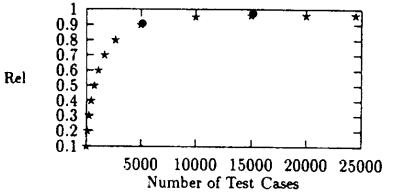
\includegraphics[width=0.48\textwidth, height= 0.2\textwidth]{figure1.PNG}
    \caption{ Project 1}
    
\end{figure}

After the .9 level was reached, in all five cases, the increase in reliability was clearly significantly slower. In particular, for Project I, the next 19,478 test cases accounted for an increase in reliability of 0.06. For Project 2, the next 51 test cases accounted for an increased reliability of 0.07, while for Project 3, the next 82 test cases accounted for an increased reliability of 0.09. For Project 4, the next 3,703 test cases accounted for an increased reliability of 0.08, while for Project 5, 22,860 additional test cases, contributed only 0.09 to the reliability. This clearly indicates a cost-benefit trade off that is worth further investigation, and is at least indicative of a testing strategy when resources are very limited, and testing must be curtailed sooner than would otherwise be desirable. 

\begin{figure}[ht]
    \centering
    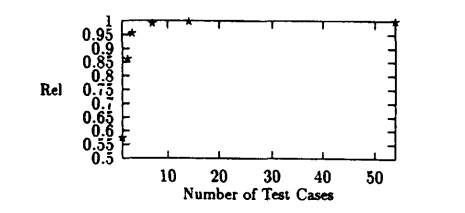
\includegraphics[width=0.48\textwidth, height= 0.2\textwidth]{figure2.PNG}
    \caption{ Project 2}
\end{figure}

\begin{figure}[ht]
    \centering
    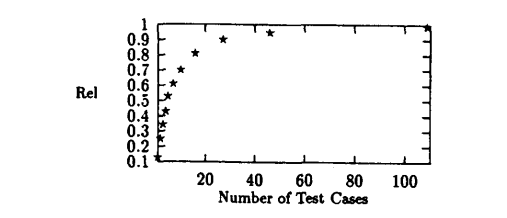
\includegraphics[width=0.48\textwidth, height= 0.2\textwidth]{figure3.PNG}
    \caption{ Project 3}
\end{figure}


\begin{figure}[ht]
    \centering
    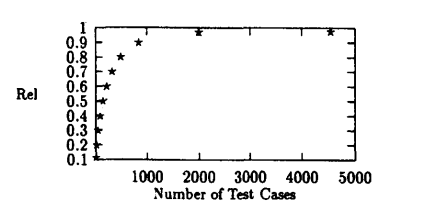
\includegraphics[width=0.48\textwidth, height= 0.2\textwidth]{figure4.PNG}
    \caption{ Project 4}
\end{figure}

\begin{figure}[ht]
    \centering
    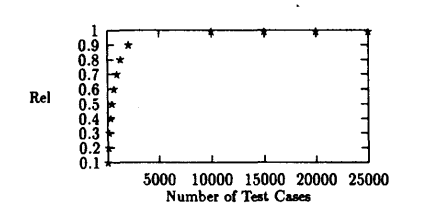
\includegraphics[width=0.48\textwidth, height= 0.2\textwidth]{figure5.PNG}
    \caption{ Project 5}
\end{figure}
It may also provide useful insights for test planning, and the initial establishment of schedules. In particular, since by using Formula 5, we are able to analytically compute the reliability
of the software relative to a given test suite without actually
running the software, we can use that computation to help the
tester determine the minimal amount of testing necessary to
guarantee a certain level of reliability assuming that there is no
operation loss. Notice that we are not suggesting that we assess
the reliability of the software without running the software on
the test suite. We are merely saying that it can be useful to get
an upper bound on the value of reliability that our measure will
provide, simply by assuming that all test cases run perfectly. In
that case, the reliability is just the amount of the probability
mass that has been covered by the test suite. If a test suite covers very little of the probability mass representing the operational profile, then very little evidence has been presented to
the user that the software is likely to perform acceptably in
their environment. It does not indicate that the software will
behave poorly, only that the testing is not sufficient to warrant
user confidence.

\subsection{Failure Severity Classification }
There are essentially two reasons why multi-user software
systems, such as the types of telecommunications systems we
studied, might experience the loss of calls (or other inputs) to
the system. The first situation happens when a burst of activity
occurs, requiring more resources than the system has available.
In the case of telecommunications systems, if the total number
of active calls plus the number of incoming calls exceeds the
system's capacity, some calls will be lost. Once the load decreases, the system resumes normal operation. Of course, even
though no actual failures have occurred, from the user's perspective, there has been a decrease in reliability, since the call
they tried to place was not completed, and this is reflected in
our reliability computation. 

The second situation occurs when there is a fault in the system. In this case, calls (or users) are lost to the system, even
though there are ample resources available. It is this type of
fault condition that is of interest here. 

One of the advantages of being able to compute a reliability
value corresponding to fault-free system behavior without actually running the software, is that it provides a baseline that
can be used for comparison for a given operational profile and
test suite. Therefore, when a system fails on some elements of
a test suite, the reliability can be computed for the faulty version of the system. At the same time, we can compute the reliability of the same test suite assuming the system performed
flawlessly. This difference in reliability computation can then
be used as the basis for an individualized notion of failure severity, where failure severity is often categorized according to
the impact on the system availability. For example one might
define a Severity 1 fault to mean that the system is totally unavailable, a Severity 2 to mean that a major system degradation has occurred, and so forth. 

Of course, in some environments, the loss of any operations,
even the most minimal amount, is intolerable. In other environments, in contrast, a significant amount of operations can
be lost before the user considers the failure severe. Thus the
same amount or percentage decrease in the computed reliability for a given fault might be rated as a severity 1 failure by
one project and as a severity 2 or 3 failure by another. 

\section{CONCLUSIONS}
In this paper, we have presented three algorithms for automatically generating test suites to test the resource allocation
behavior of software systems that are model able by Markov
chains. We have built a tool that does the automatic test suite
generation and used it to generate suites for five large industrial software telecommunications systems. These initial results
are extremely encouraging, with projects reporting the detection of serious program faults that they predict would not have
been detected until field release, had these algorithms not been
used. They also report a greatly facilitated regression testing
and fault localization capability due to the use of these
algorithms. 

We also introduced a new approach to software reliability to
be used to assess software that has been tested using our load
testing algorithms, and applied this definition to assess the
reliability of the five industrial systems we tested. Since all of
the systems that we tested were designed to run at low to medium utilization rates, it therefore follows that the amount of
excess capacity available in these systems makes it unlikely
that there will be many failures encountered in practice, even
when the system is running in a degraded state. For this reason,
we investigated the effects on the reliability computation of
varying degrees of system degradation relative to a particular
operational distribution. We have applied this approach to
assess the five industrial telecommunications projects for
which we generated test suites, and presented data showing the
expected reliability for each project under different circumstances. We have also considered two possible applications of
our reliability measure. In the first case, we discussed the use
of the reliability notion to track the progress of our load testing
algorithms, and to use it to guide test planning. We also proposed a way to use our reliability notion to guide the user in
the assessment of the severity of observed failures. 

We are very encouraged by the plausibility of our initial results. In each case, the results that we obtained when computing the reliability of systems relative to a particular operational
distribution, were consistent with our intuitive expectations.
We therefore intend to continue applying our notion of reliability to other industrial projects, as they reach the load testing phase of development, after we apply our algorithms to
generate test suites. We are optimistic that the combination of
our automatic test suite generation algorithms, and the application of our approach to reliability assessment and reliability based system test tracking, will be very useful for projects that
can be appropriately modeled. 

Because we have derived a relationship between the reliability of smoothly degrading systems, and the operational
distribution, it should be possible to consider the incremental
calculation of reliability for projects as their operational distributions change due to changes in the system requirements, or
as a reflection of the environmental conditions of a new customer. We also plan to consider the application of these notions to domains other than telecommunications systems. 

\begin{thebibliography}{}
\bibitem{b1}A. Avritzer and B. Larson, “Load testing software using deterministic
state testing,” T. Ostrand and E. Weyuker, eds., Proc. of the 1993 Int’I
Symp. on Software Testing and Analysis (ISSTA). ACM Press, June 1993, pp. 82-88.

\bibitem{b2}J.W. Duran and S.C. Ntafos, “An evaluation of random testing.” IEEE
Transactions on Software Engineering, vol. 10, no. 4, July 1984, pp.
438444. 

\bibitem{b3}P.G. Frank1 and E.J. Weyuker, “Provable improvements on branch
testing,” IEEE Transactions on Software Engineering, vol. 19, no. 10, Oct. 1993, pp. 962-975. 

\bibitem{b4}R. Hamlet and R. Taylor, “Partition testing does not inspire confidence,” Proc. Second Workshop on Software Testing, Verification, and
Analysis, Banff, Canada, Ju!y 1988, pp. 206-215. 

\bibitem{b5}L. Kleinrock, Queueing Systems, Volume 1: Theory. New York: WileyInterscience, 1975. 

\bibitem{b6}J.D. Musa, A. Iannino, and K. Okumoto, Software Reliability Measurement, Prediction, Application. New York: McGraw-Hill, 1987. 

\bibitem{b7}J.D. Musa, “Operational profiles in software reliability engineering,”
IEEE Software, vol. IO, no. 2, Mar. 1993, pp. 14-32. 

\bibitem{b8}T.A. Thayer, M. Lipow, and E.C. Nelson, Software Reliability. New
York: North-Holland, 1978. 

\bibitem{b9}S.N. Weiss and E. Weyuker, “An extended domain-based model of
software reliability,” IEEE Transactions on Software Engineering, vol.
14, no. 10, Oct. 1988, up. 1,512-1.524. 

\bibitem{b10}E.J. Weyuker and B. Jeng, “Analyzing partition testing strategies,”
IEEE Transactions on Software Engzneering, vol. 17, no. 7, July 1991, pp. 703-7 1 1. 

\bibitem{b11}E.J. Weyuker and T.J. Ostrand, “Theories of program testing and the
application of revealing subdomains,” IEEE Transactions on Software
Engineering, vol. 6, no. 3, Mar. 1980, pp. 23&245. 



\end{thebibliography}



\textit{Alberto Avriher} received a PhD in computer science from the University of California, Los Angeles,
an MSc in computer science from the Federal University of Minas Gerais, Brazil, and the BSc in
computer engineering from the Technion, Israel
lnstitute of Technology. He is currently a member of
the technical staff in the Operations Technology
Center at AT&T Bell Labofatories at Middletown,
N.J. He spent the summer of 1987 at IBM Research
at Yorktown Heights His research interests are in
software engineering, particularly software testing
and reliability, real-time systems, and performance modeling, and has published several papers in those areas. He is a member of ACM SIGSOFT and
IEEE. 

\textit{Elaine Weyuker} received a PhD in computer science from Rutgers University, and an MSE from the
Moore School of Electrical Engineering, University
of Pennsylvania. She is currently a distinguished
member of the technical staff in the Software and
Systems Research Center at AT&T Bell Laboratories
at Murray Hill, N.J , and a professor of computer
science at the Courant Institute of Mathematical
Sciences of New York University Before coming to
NYU, she was on the faculty of the City University
of New York, was a systems engineer for IBM, and
was a programmer for Texaco, Inc Her research interests are in software
engineering, particularly software testing and reliability, and software complexity measures, and has published many papers in those areas. She is also
interested in the theory of computation, and is the author of a book (with
Martin Davis and Ron Sigal), Computubdity, Complexity, and Languages,
published by Academic Press, 1994. She is currently a member of the editorial board of ACM Transactions on Sofhyare Engineering and Methodologv
(TOSEM). She has been the Secretatymreasurer of ACM SIGSOFT, a member of the Executive Committee of the IEEE Computer Society Technical
Committee on Software Engineering and an ACM National Lecturer. She has
also been a member of the ACM Committee on the Status of Women and
Minorities, and of the CRA Committee on the Status of Women. 

\end{document}